\documentclass[UTF8, 16pt]{beamer}
 
% Chinese
\usepackage{xeCJK}

% Font
\usepackage{bookman}
\usefonttheme{serif}
% \usepackage[T1]{fontenc}
%\usepackage{tgbonum}

% Other packages
\usepackage{hyperref}
\usepackage{appendixnumberbeamer}
\usepackage{latexsym}
\usepackage{amsmath}
\usepackage{xcolor}
\usepackage{multicol}
\usepackage{booktabs}
\usepackage{graphicx}
\usepackage{listings}
\usepackage{stackengine}

% SUFE.sty
\usepackage{SUFE} 
% Bibtex
\usepackage[citestyle=authoryear-comp, 
            backend=biber, 
            bibstyle=numeric, 
%			sorting=ynt
            ]{biblatex}
\setbeamertemplate{bibliography item}[text]
\addbibresource{ref.bib}

% Other setting
\setlength{\parskip}{1em} % 设置段落之间的间距为 1em
\graphicspath{{res/}}
\setCJKmainfont{PingFang SC}
\setCJKmonofont{Yahei Mono}

%%%%%%%%%%%%%%%%%%%%%%%%%%

% Title page
%% Author
\author[计算机协会] % The short name
{
%Name
计算机协会
%\inst{1}
%\and
%XXX 
%\inst{2}
} 
%% Title & Subtitle
\title[Java 常规教学]{Java 常规教学}
\subtitle{}
%% Institution
\institute[SUFE]
{
%\inst{1}
% Shanghai University of Finance and Economics
上海财经大学
%\and
%\inst{2}
%Shanghai University of Finance and Economics
}
%% Date
\date{23会计学院\ ACCA\ 张华轩}
%%Logo
%\logo{
\includegraphics[height=1cm]{sufe_logo}}

%%%%%%%%%%%%%%%%%%%%%%%%%%

% Document begins
\begin{document}

%Title page
\begin{frame}[noframenumbering]
    %	\thispagestyle{empty}
    \titlepage{}
    % Logo
    \vspace{-0.5cm}
    \begin{figure}[htpb]
        \begin{center}
            
\includegraphics[width=0.19 \linewidth]{sufe_logo.png}
            \quad
            
\includegraphics[width=0.19 \linewidth]{ca_logo.png}
        \end{center}
    \end{figure}
\end{frame}

% % Contents page
% \begin{frame}{Contents}
% 	\tableofcontents[sectionstyle=show,
% 		subsectionstyle=show/shaded/hide,
% 		subsubsectionstyle=show/shaded/hide]
% \end{frame}

% Body
\section{Java生态}
\begin{frame}
    \centering
    \textcolor{sufered}{Spring \& Spring Boot}
    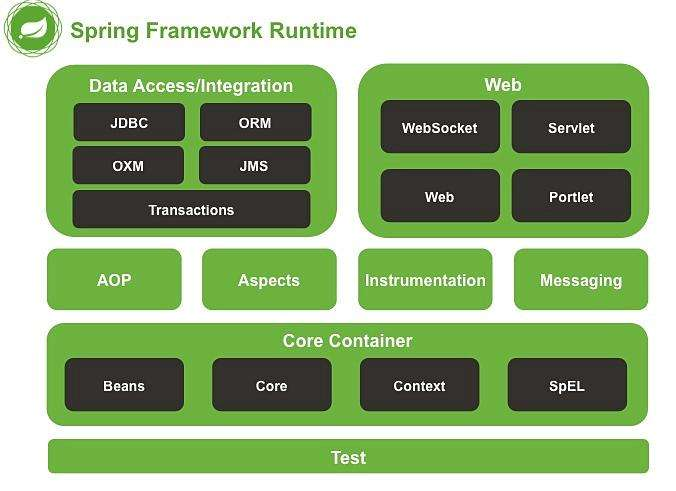
\includegraphics[width=0.95\linewidth]{ch1/spring.png}
\end{frame}

\begin{frame}
    \centering
    \textcolor{sufered}{Hadoop, Storm(Clojure), Spark(Scala)}
    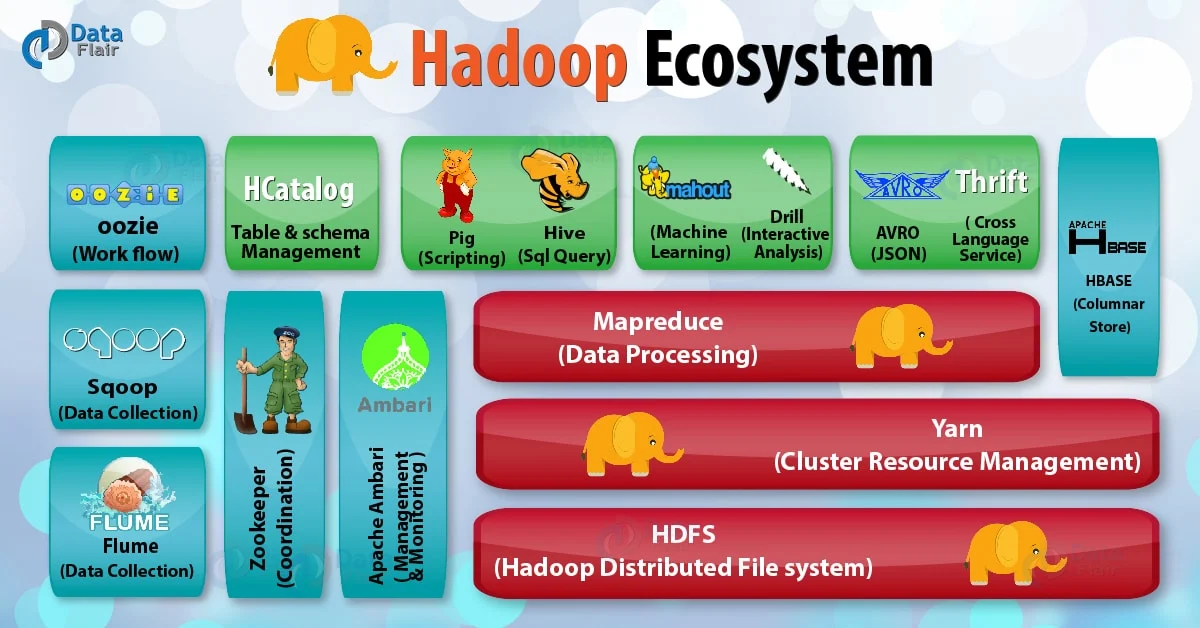
\includegraphics[width=0.95\linewidth]{ch1/hadoop.png}
\end{frame}

\begin{frame}
    \centering
    \textcolor{sufered}{Android App Development}
    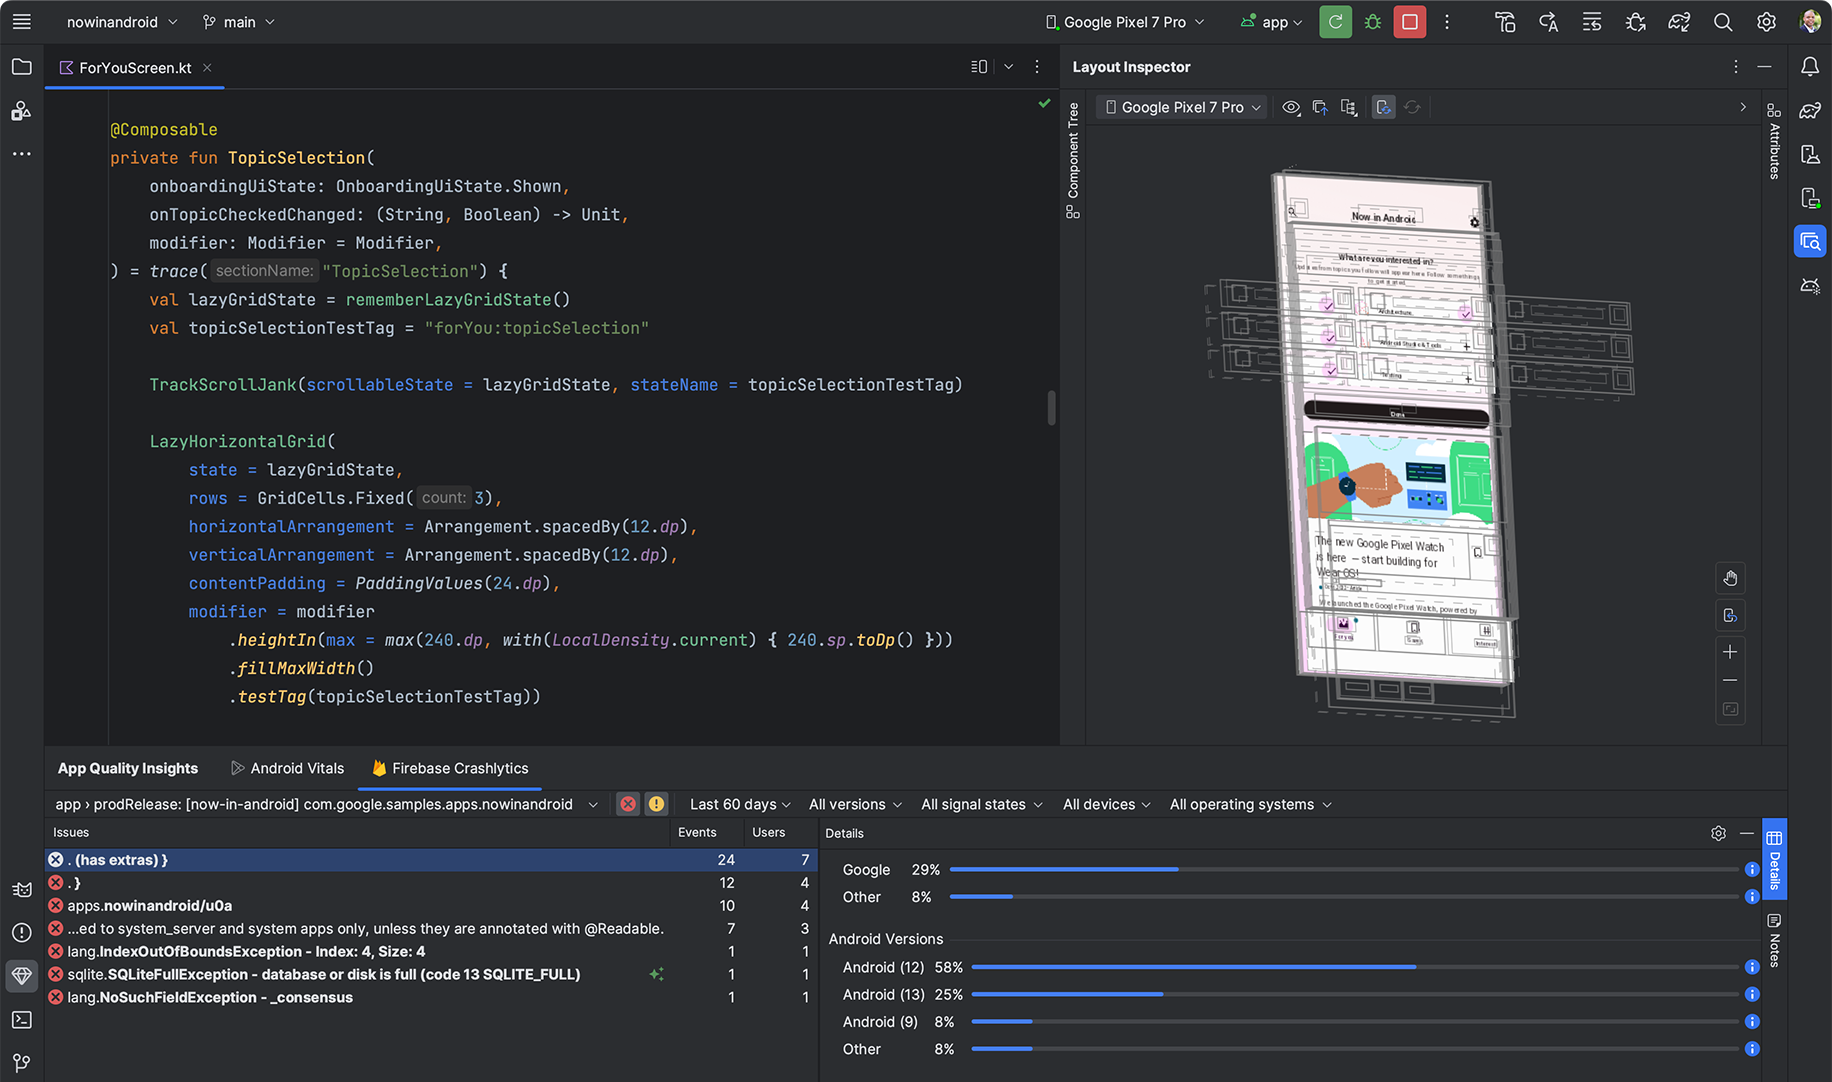
\includegraphics[width=0.95\linewidth]{ch1/as.png}
\end{frame}

\section{Java基础}
\begin{frame}
    \frametitle{环境配置}
    \textcolor{sufered}{?有必要吗}

    \textcolor{sufered}{谁还用命令行编译Java}

    \begin{itemize}
        \item \texttt{JRE(Java Runtime Environment)}:Java运行时环境
        \item \texttt{JDK(Java Development Kit)}:Java开发工具包
        \item \texttt{Java IDE}:Eclipse, IntelliJ IDEA, VS Code(new!)
    \end{itemize}

    \url{https://www.jetbrains.com/zh-cn/idea}

    \textcolor{sufered}{IntelliJ启动!}
\end{frame}

\begin{frame}
    \centering
    \textcolor{sufered}{Java版本演进}
    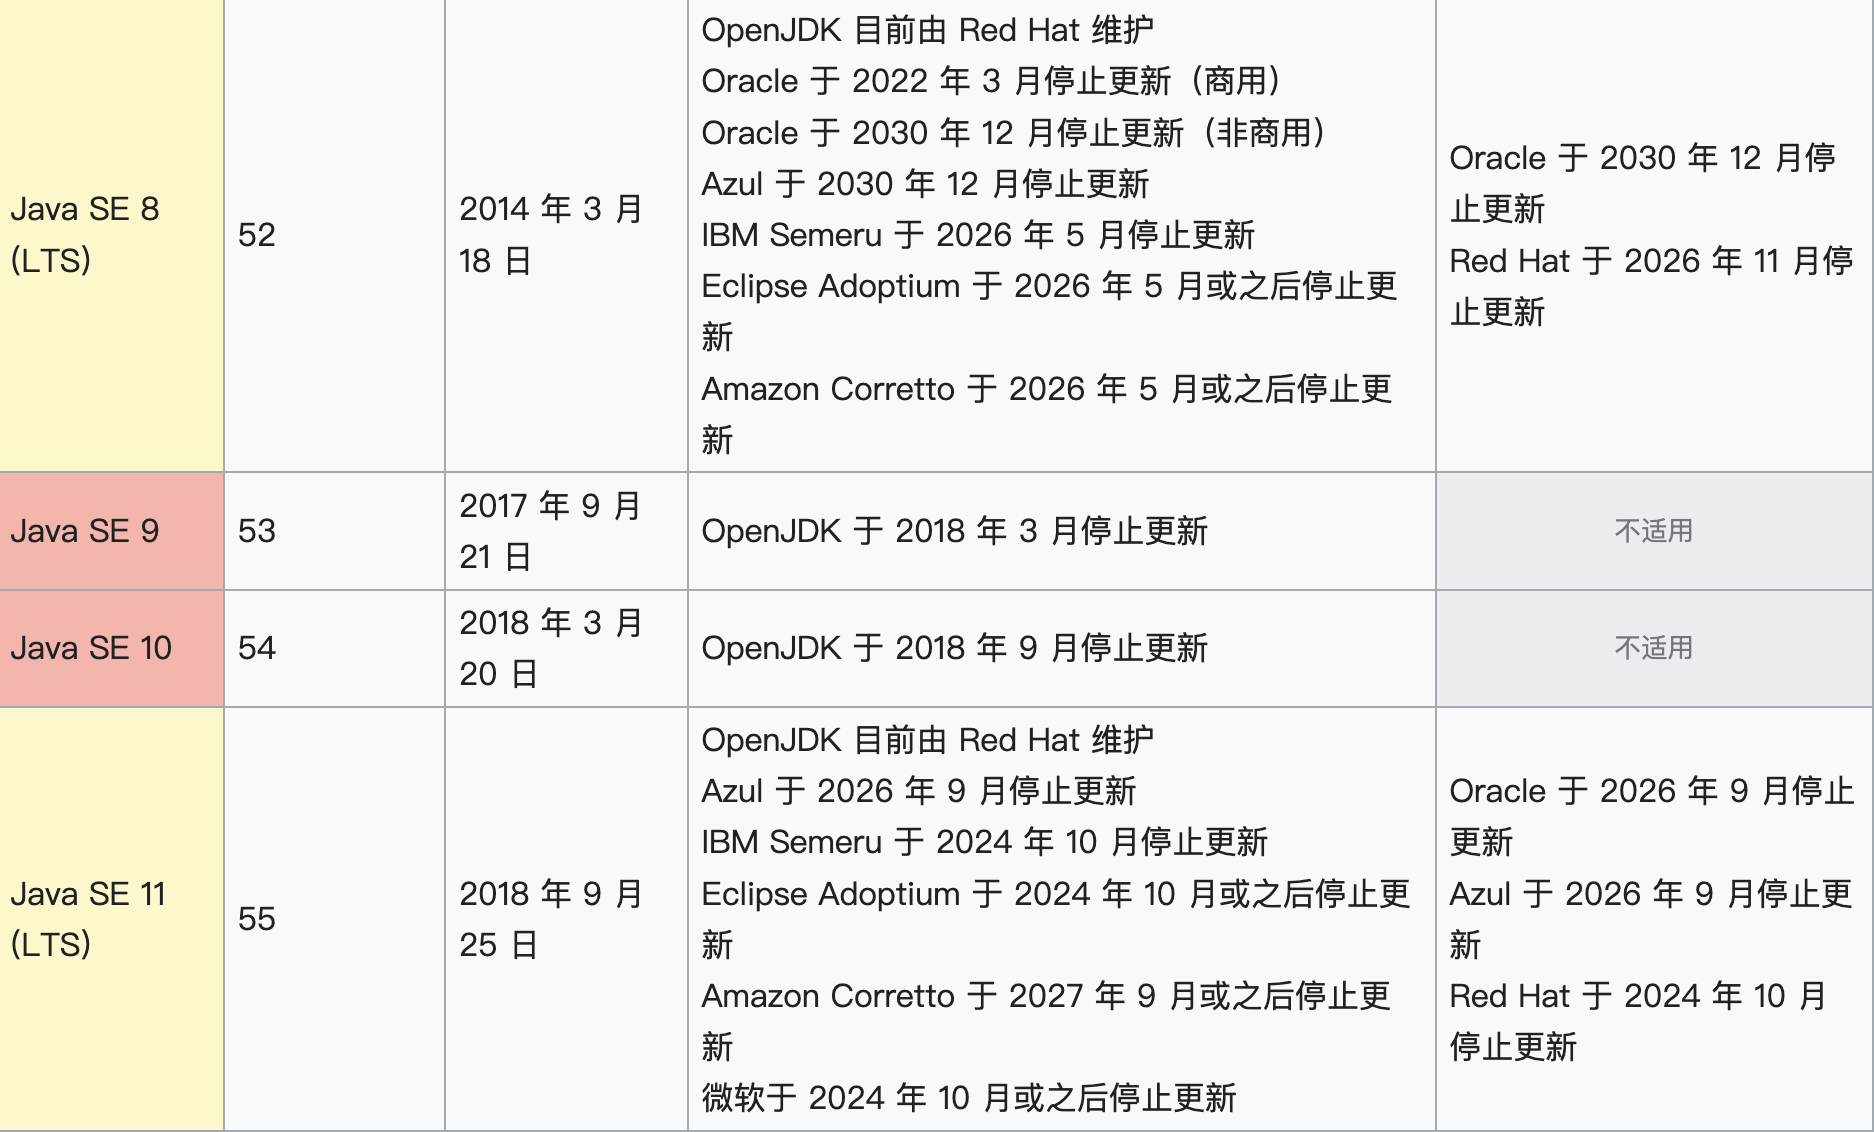
\includegraphics[width=0.95\linewidth]{ch1/edition.png}
    \texttt{Latest: Java SE 25(LTS)}
\end{frame}

\begin{frame}
    \frametitle{JDK}
    \textcolor{sufered}{主流JDK分支}

    \begin{itemize}
        \item \texttt{OpenJDK}:由社区支持、开源
        \item \texttt{Oracle JDK}:Oracle主导、商用(最后的免费商用版本是8u202)
        \item \texttt{Adoptium Eclipse Temurin}:由Eclipse基金会支持、开源
        \item \texttt{Amazon Corretto}:由Amazon主导、免费商用
    \end{itemize}

    \url{https://adoptium.net/zh-CN/temurin/releases}
\end{frame}

\begin{frame}[fragile]
    \frametitle{JVM}
    \textcolor{sufered}{Java虚拟机(Java Virtual Machine)}
    \begin{itemize}
        \item \texttt{是什么}:用于执行Java字节码的虚拟机,拥有独立的运行机制,所有Java程序都运行在JVM内部,但其运行的Java字节码未必由Java编译而成
        \item \texttt{为什么}:一次编译,到处运行;自动内存管理;自动垃圾回收功能(GC)
        \item \texttt{怎么样}:汇编->字节码,本地运行时->JVM运行时,只需要针对特定平台提供JVM实现
    \end{itemize}

    \textcolor{sufered}{JVM对内提供统一接口,对外对接本地接口}
\end{frame}

\begin{frame}
    \centering
    \textcolor{sufered}{Java虚拟机运行时}
    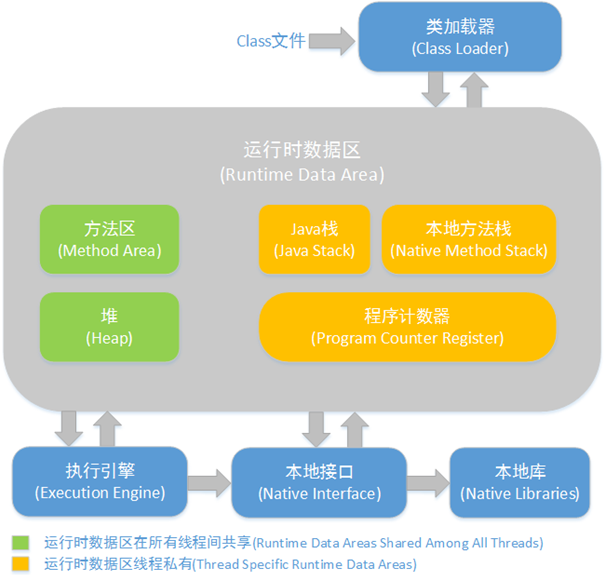
\includegraphics[width=0.75\linewidth]{ch1/jvm.jpg}
\end{frame}

\begin{frame}[fragile]
    \frametitle{基本结构}
    \textcolor{sufered}{最简单的类}
    \begin{lstlisting}
/**
* 可以用来自动创建文档的注释
**/
public class Solution {
    public static void main(String[] args) {
        // 向屏幕输出文本:
        System.out.println("Hello, world!");
        /* 多行注释开始
        注释内容
        注释结束 */
    }
} // class定义结束
    \end{lstlisting}
\end{frame}

\begin{frame}
    \frametitle{基本结构}
    \textcolor{sufered}{Annotation for Cpp}

    \begin{itemize}
        \item \textbf{入口方法}:main方法为入口方法,是程序的唯一入口
        \item \textbf{外壳类(shell class)}:Solution类在这里没有任何作用
        \item \textbf{退出码(exit code)}:main方法不返回任何值
    \end{itemize}

    \textcolor{sufered}{任何Java源文件都是类/类的集合!}
\end{frame}

\begin{frame}
    \frametitle{Dive-in}
    \textcolor{sufered}{入口方法}

    \begin{itemize}
        \item \textbf{public修饰符}:main方法是唯一的程序入口,为了让JVM可以调用,必须使用public修饰符暴露出来
        \item \textbf{static静态方法}:入口方法需要在类创建之前调用
        \item \textbf{void返回值}:JVM不接受返回值,所以返回void
    \end{itemize}
\end{frame}

\begin{frame}
    \frametitle{Java访问修饰符}
    \textcolor{sufered}{访问修饰符}

    \begin{itemize}
        \item \textbf{public}:公共访问,允许该类或成员被任何其他类访问
        \item \textbf{protected}:受保护访问,仅限于同包内的类和子类
        \item \textbf{包访问}:不加修饰符时,默认包访问,仅限同包内访问
        \item \textbf{private}:私有访问,仅限类内部访问。适用于不希望外部直接访问的属性或方法
    \end{itemize}
\end{frame}

\begin{frame}[fragile]
    \frametitle{Example}
    \textcolor{sufered}{protected子类访问}

    \begin{lstlisting}
class Parent {
    protected String message = "Hello from Parent";

    protected void displayMessage() {
        System.out.println(message);
    }
}

class Child extends Parent {
    public void show() {
        displayMessage(); // 子类可以访问父类的受保护方法
    }
}
    \end{lstlisting}
\end{frame}

\begin{frame}[fragile]
    \frametitle{Example(Continue)}
    \textcolor{sufered}{protected子类访问}
    \begin{lstlisting}
public class Main {
    public static void main(String[] args) {
        Child child = new Child();
        child.show(); // 输出: Hello from Parent
    }
}
    \end{lstlisting}
\end{frame}

\begin{frame}[fragile]
    \frametitle{Example}
    \textcolor{sufered}{protected包内访问}

    \begin{lstlisting}
package mypackage;
class Parent {
    protected String message = "Hello from Parent";

    protected void displayMessage() {
        System.out.println(message);
    }
}

class NonSubclass {
    public void accessParent() {
        Parent parent = new Parent();
        parent.displayMessage(); // 可访问包内的受保护方法
    }
}
        \end{lstlisting}
\end{frame}

\begin{frame}[fragile]
    \frametitle{Example(Continue)}
    \textcolor{sufered}{protected包内访问}

    \begin{lstlisting}
public class Main {
    public static void main(String[] args) {
        NonSubclass example = new NonSubclass();
        example.accessParent(); // 输出: Hello from Parent
    }
}
    \end{lstlisting}
\end{frame}

\begin{frame}
    \frametitle{Why protected?}
    \textcolor{sufered}{Annotation for Cpp}

    \begin{itemize}
        \item \textbf{Java}:同包内的类和子类均可以访问
        \item \textbf{C++}:仅限子类访问
    \end{itemize}

    \texttt{Java访问修饰符的设计大体参考C++}

    \textcolor{sufered}{为什么允许包内访问?}
\end{frame}

\begin{frame}[fragile]
    \frametitle{Java 包机制}
    \textcolor{sufered}{Java Package}

    \begin{itemize}
        \item \textbf{包的定义}:Java 包(Package)是一种命名空间机制,用于将相关的类和接口分组

        \item \textbf{包的作用}:
              \begin{itemize}
                  \item \textbf{命名空间}:提供独立的命名空间,防止类和接口命名冲突
                  \item \textbf{访问控制}:包允许定义类和成员的访问级别(public、protected、default和private),实现不同的封装级别。
                  \item \textbf{模块化}:将相关的类按功能分组,建立模块化的项目结构
              \end{itemize}
    \end{itemize}
\end{frame}

\begin{frame}[fragile]
    \frametitle{Example}
    \textcolor{sufered}{Java Package}
    \begin{lstlisting}
// 在 mypackage 包中定义一个类
package mypackage;

public class MyClass {
    public void display() {
        System.out.println("Hello from MyClass in mypackage");
    }
}

// 在其他类中导入该包
import mypackage.MyClass;
    \end{lstlisting}
\end{frame}


\begin{frame}
    \frametitle{设计模式:组合}
    \textcolor{sufered}{组合而非继承}

    \texttt{组合模型中,一个对象(称为复合对象)可以包含另一个对象(称为组件对象),复合对象可以使用组件对象的行为}

    \textcolor{sufered}{降低继承可能带来的耦合性}
\end{frame}

% \section{Vim 编辑器}
% \begin{frame}
%     123
% \end{frame}

% \section{Git 版本控制}
% \begin{frame}
%     123
% \end{frame}

% \section{正则表达式}
% \begin{frame}
%     123
% \end{frame}

% \section{SH 脚本}
% \begin{frame}
%     123
% \end{frame}

%%%%%%%%%%%%%%%%%%%%%%%%%%

% End
\begin{frame}[allowframebreaks]%{End}
    \begin{center}
        \Huge\textbf{\textit{\texttt{Thanks!}}}
    \end{center}
\end{frame}

% Reference
\appendix
\begin{frame}{Reference}
    \nocite{corejava}
    \nocite{liaoxuefeng}
    \addtocounter{framenumber}{-1}
    \printbibliography{} % [heading=bibintoc, title=Reference]
\end{frame}

%%%%%%%%%%%%%%%%%%%%%%%%%%

% Snippets
% \begin{frame}[noframenumbering, plain]{Snippets}
%     \begin{multicols}{2}
%         \begin{enumerate}
%             \item 123~\cite[Page10]{corejava}
%         \end{enumerate}
%         \begin{itemize}
%             \item \[V = \frac{4}{3}\pi r^3\]
%             \item $ V = \frac{4}{3}\pi r^3 $
%         \end{itemize}
%     \end{multicols}
%     \begin{equation}
%         \label{eq1}
%         V = \frac{4}{3}\pi r^3
%     \end{equation}
%     \center{}
%     As Equation (\ref{eq1}) \textcolor{sufered}{shows},
%     $\cdots$, this \emph{equation} is \alert{important}.
% \end{frame}

% \begin{frame}[noframenumbering, plain]{Snippets}
%     \begin{columns}
%         \column{0.5\textwidth}
%         \begin{block}{Remark}
%             Sample text
%         \end{block}
%         \begin{alertblock}{Important theorem}
%             red box
%         \end{alertblock}
%         \begin{examples}
%             Sample text in green box.
%         \end{examples}
%         \column{0.5\textwidth}
%         \begin{table}
%             \centering
%             \caption{caption}
%             % \vspace{-0.5cm}
%             \setlength{\tabcolsep}{5mm}
%             {
%                 \begin{tabular}{lcc}
%                     \toprule %\hline
%                     1234                     & 123       & a \\ \midrule
%                     \textcolor{deepred}{135} & w         & f \\
%                     \textcolor{sufered}{126} & \alert{a} & d \\ \bottomrule
%                 \end{tabular}
%             }
%         \end{table}
%     \end{columns}
% \end{frame}
%\backupend
%%%%%%%%%%%%%%%%%%%%%%%%%%
\end{document}